% NB: use pdflatex to compile NOT pdftex.  Also make sure youngtab is
% there...

% converting eps graphics to pdf with ps2pdf generates way too much
% whitespace in the resulting pdf, so crop with pdfcrop
% cf. http://www.cora.nwra.com/~stockwel/rgspages/pdftips/pdftips.shtml




\documentclass[10pt,aspectratio=169,dvipsnames]{beamer}

\usetheme[color/block=transparent]{metropolis}

\usepackage[absolute,overlay]{textpos}
\usepackage{booktabs}
\usepackage[utf8]{inputenc}


\usepackage[scale=2]{ccicons}

\usepackage[official]{eurosym}

%use this to add space between rows
\newcommand{\ra}[1]{\renewcommand{\arraystretch}{#1}}


\setbeamerfont{alerted text}{series=\bfseries}
\setbeamercolor{alerted text}{fg=Mahogany}
\setbeamercolor{background canvas}{bg=white}


\newcommand{\R}{\mathbb{R}}

\def\l{\lambda}
\def\m{\mu}
\def\d{\partial}
\def\cL{\mathcal{L}}
\def\co2{CO${}_2$}


\def\bra#1{\left\langle #1\right|}
\def\ket#1{\left| #1\right\rangle}
\newcommand{\braket}[2]{\langle #1 | #2 \rangle}
\newcommand{\norm}[1]{\left\| #1 \right\|}
\def\corr#1{\Big\langle #1 \Big\rangle}
\def\corrs#1{\langle #1 \rangle}



% for sources http://tex.stackexchange.com/questions/48473/best-way-to-give-sources-of-images-used-in-a-beamer-presentation

\setbeamercolor{framesource}{fg=gray}
\setbeamerfont{framesource}{size=\tiny}


\newcommand{\source}[1]{\begin{textblock*}{5cm}(10.5cm,8.35cm)
    \begin{beamercolorbox}[ht=0.5cm,right]{framesource}
        \usebeamerfont{framesource}\usebeamercolor[fg]{framesource} Source: {#1}
    \end{beamercolorbox}
\end{textblock*}}

\usepackage{hyperref}


\usepackage{tikz}
\usetikzlibrary{arrows.meta}


\usepackage[europeanresistors,americaninductors]{circuitikz}


%\usepackage[pdftex]{graphicx}


\graphicspath{{graphics/}}

\DeclareGraphicsExtensions{.pdf,.jpeg,.png,.jpg,.gif}



\def\goat#1{{\scriptsize\color{green}{[#1]}}}



\let\olditem\item
\renewcommand{\item}{%
\olditem\vspace{5pt}}

\title{Energy System Modelling\\ Summer Semester 2020, Lecture 4}
%\subtitle{---}
\author{
  {\bf Dr. Tom Brown}, \href{mailto:tom.brown@kit.edu}{tom.brown@kit.edu}, \url{https://nworbmot.org/}\\
  \emph{Karlsruhe Institute of Technology (KIT), Institute for Automation and Applied Informatics (IAI)}
}

\date{}

\titlegraphic{
  \vspace{0cm}
  \hspace{10cm}
    \includegraphics[trim=0 0cm 0 0cm,height=1.8cm,clip=true]{kit.png}

\vspace{5.1cm}

  {\footnotesize

  Unless otherwise stated, graphics and text are Copyright \copyright Tom Brown, 2020.
  Graphics and text for which no other attribution are given are licensed under a
  \href{https://creativecommons.org/licenses/by/4.0/}{Creative Commons
  Attribution 4.0 International Licence}. \ccby}
}

\begin{document}

\maketitle


\begin{frame}

  \frametitle{Table of Contents}
  \setbeamertemplate{section in toc}[sections numbered]
  \tableofcontents[hideallsubsections]
\end{frame}



\section{3-node example from last time}


\begin{frame}
  \frametitle{Solving 3-node example}

  Last time we looked at an example where energy conservation at each
  vertex (Kirchhoff's Current Law, KCL) was not enough information to
  solve the power flow, since there are multiple paths in the network.
  Assume equal reactances $x_\ell = x$ on each edge.

  \vspace{.3cm}

  \begin{columns}
    \column[c]{.5\textwidth}


    \centering

  %https://tex.stackexchange.com/questions/270543/draw-a-graph-in-latex-with-tikz
  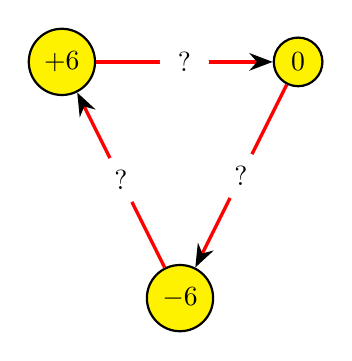
\begin{tikzpicture}
    \begin{scope}[every node/.style={circle,thick,draw,fill=yellow}]
      \node (1) at (0,3) {$+6$};
      \node (2) at (3,3) {$0$};
      \node (3) at (1.5,0) {$-6$};
    \end{scope}

    \begin{scope}[>={Stealth[black]},
        every node/.style={fill=white,circle},
        every edge/.style={draw=red,very thick}]
      \path [->] (1) edge node {$?$} (2);
      \path [->] (2) edge node {$?$} (3);
      \path [->] (3) edge node {$?$} (1);
    \end{scope}
  \end{tikzpicture}


      \column[c]{.5\textwidth}

      Formalise by labelling the nodes and edges:

      \vspace{.5cm}

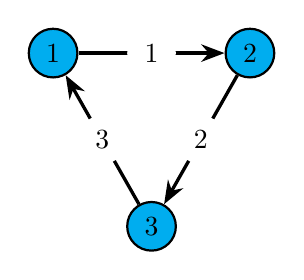
\begin{tikzpicture}
    \begin{scope}[every node/.style={circle,thick,draw,fill=cyan}]%text=white}]
      \node (1) at (0,2.5) {1};
      \node (2) at (2.5,2.5) {2};
      \node (3) at (1.25,.3) {3};
    \end{scope}

    \begin{scope}[>={Stealth[black]},
        every node/.style={fill=white,circle},
        every edge/.style={draw=black,very thick}]
      \path [->] (1) edge node {1} (2);
      \path [->] (2) edge node {2} (3);
      \path [->] (3) edge node {3} (1);
    \end{scope}
  \end{tikzpicture}

      \vspace{.5cm}

We have $p_i = (6,0,-6)$. (Check $\sum_i p_i = 0$.)

Goal is to find $f_\ell$ for $\ell = 1,2,3$.

  \end{columns}
\end{frame}



\begin{frame}
  \frametitle{Solving 3-node example: Kirchhoff's Current Law (KCL)}
  \begin{columns}

      \column[c]{.5\textwidth}

      \vspace{.2cm}

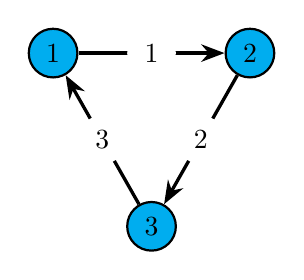
\begin{tikzpicture}
    \begin{scope}[every node/.style={circle,thick,draw,fill=cyan}]%text=white}]
      \node (1) at (0,2.5) {1};
      \node (2) at (2.5,2.5) {2};
      \node (3) at (1.25,.3) {3};
    \end{scope}

    \begin{scope}[>={Stealth[black]},
        every node/.style={fill=white,circle},
        every edge/.style={draw=black,very thick}]
      \path [->] (1) edge node {1} (2);
      \path [->] (2) edge node {2} (3);
      \path [->] (3) edge node {3} (1);
    \end{scope}
  \end{tikzpicture}

      \vspace{.3cm}

      Kirchhoff's Current Law gives us:
  \begin{equation*}
    p_i = \sum_\ell K_{i\ell} f_\ell \hspace{2cm} \forall i
  \end{equation*}

  The incidence matrix $K$ is given by:
        \begin{equation*}
\mathbf{K}_{i \ell}=\left(\begin{matrix}
 1 & 0 & -1\\
 -1 & 1 & 0\\
 0 & -1 & 1
\end{matrix}\right)
\end{equation*}
      \column[c]{.5\textwidth}
        So we get:
        \begin{align*}
          p_1 & = 6 = f_1 - f_3 \\
          p_2 & = 0 = f_2 - f_1 \\
          p_3 & = -6 = f_3 - f_2
        \end{align*}
        Sum of KCL equations is always zero, so
        reduce to $N-1 = 2$ independent equations:
        \begin{align*}
          6 & = f_1 - f_3 \\
          0 & = f_2 - f_1
        \end{align*}
        Not enough information to solve!

        Need more information from KVL and reactances.

  \end{columns}
\end{frame}






\begin{frame}
  \frametitle{Solving 3-node example: Kirchhoff's Voltage Law (KVL)}
  \begin{columns}

      \column[c]{.5\textwidth}

      \vspace{.2cm}

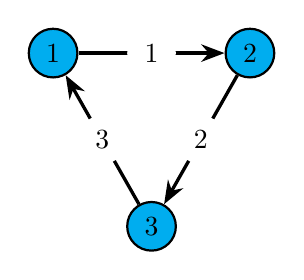
\begin{tikzpicture}
    \begin{scope}[every node/.style={circle,thick,draw,fill=cyan}]%text=white}]
      \node (1) at (0,2.5) {1};
      \node (2) at (2.5,2.5) {2};
      \node (3) at (1.25,.3) {3};
    \end{scope}

    \begin{scope}[>={Stealth[black]},
        every node/.style={fill=white,circle},
        every edge/.style={draw=black,very thick}]
      \path [->] (1) edge node {1} (2);
      \path [->] (2) edge node {2} (3);
      \path [->] (3) edge node {3} (1);
    \end{scope}
  \end{tikzpicture}

      \vspace{.1cm}

      One formulation of Kirchhoff's Voltage Law gives us $L-N+1$ equations for cycles:
  \begin{equation*}
    \sum_\ell C_{\ell c} x_\ell f_\ell = 0 \hspace{2cm} \forall c
  \end{equation*}
  The cycle matrix $C$ is given by:
        \begin{equation*}
\mathbf{C}_{\ell c}=\left(\begin{matrix}
 1 \\
 1\\
 1
\end{matrix}\right)
\end{equation*}
      \column[c]{.5\textwidth}
        For equal reactances $x_\ell = x$ we get:
        \begin{align*}
          \sum_\ell C_{\ell 1} x_\ell f_\ell = x(f_1 + f_2 + f_3) = 0
        \end{align*}
        Together with KCL equations we now have 3 independent equations for 3 unknowns. Solve:
        \begin{align*}
          f_1 & = 2 \\
          f_2 & = 2 \\
          f_3 & = -4
        \end{align*}

  \end{columns}
\end{frame}




\begin{frame}
  \frametitle{Solving 3-node example: Solution}

  \vspace{.3cm}

  \begin{columns}

      \column[c]{.5\textwidth}

  Solution:
  \vspace{.3cm}

    \centering
  %https://tex.stackexchange.com/questions/270543/draw-a-graph-in-latex-with-tikz
  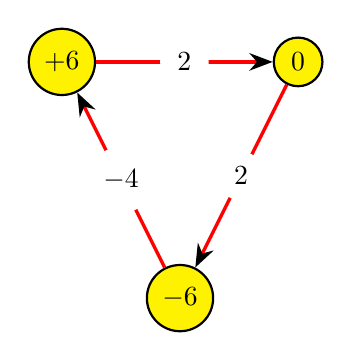
\begin{tikzpicture}
    \begin{scope}[every node/.style={circle,thick,draw,fill=yellow}]
      \node (1) at (0,3) {$+6$};
      \node (2) at (3,3) {$0$};
      \node (3) at (1.5,0) {$-6$};
    \end{scope}

    \begin{scope}[>={Stealth[black]},
        every node/.style={fill=white,circle},
        every edge/.style={draw=red,very thick}]
      \path [->] (1) edge node {$2$} (2);
      \path [->] (2) edge node {$2$} (3);
      \path [->] (3) edge node {$-4$} (1);
    \end{scope}
  \end{tikzpicture}

  \raggedright

      \column[c]{.5\textwidth}

      Along 2-edge path reactance is double the 1-edge path, so half as much power flows along the 2-edge path as the 1-edge path.

      \vspace{.5cm}
  NB: For directed graph, sign determines direction of flow.

  \end{columns}
\end{frame}




\section{Full power flow equations}


\begin{frame}
  \frametitle{Goal: Understand the physical origin of these equations}

  Last time we said we can (in the linear approximation) express the
  flow $f_\ell$ on each line in terms of the voltage angles $\theta_i$
  at the nodes for a line $\ell$ with
  reactance $x_\ell$ as
  \begin{equation*}
    f_\ell = \frac{\theta_i - \theta_j}{x_\ell} = \frac{1}{x_\ell}\sum_{i} K_{i\ell} \theta_i
  \end{equation*}
   This is a relative of Ohm's Law in DC circuits, $I = \frac{V_1 - V_2}{R}$.


  Now we explain the physics of where this comes from, and the linear approximation
  that leads to it.

  This is also useful when we consider the synchronisation of
  oscillators later.
\end{frame}


\begin{frame}
  \frametitle{Alternating Current}

  The majority of electrical power, including what you get out of a
  wall plug, is transmitted as \alert{Alternating Current (AC)},
  i.e. both the voltage and current are sinusoidal waves.

  \begin{center}
  \includegraphics[width=8cm]{738px-Types_of_current}
  \end{center}

  [Some power is transmitted as \alert{Direct Current (DC)} under bodies of water and
    indeed many electronic devices require DC (must convert AC to DC).]
  \source{Wikipedia}
\end{frame}




\begin{frame}
  \frametitle{Why alternating current?}

  Battle of currents! Edison versus Westinghouse/Tesla in late 1880s, early 1890s, etc.

  \url{https://en.wikipedia.org/wiki/War_of_Currents}

  AC won, because it's easy to transform AC to a higher voltage, so
  you can transmit a given power $P = VI$ with a lower current and thus avoid
  the $I^2R$ resistive losses in power lines.

  Reason: $\frac{d}{dt}$ in $\mathcal{E} = \frac{d\Phi}{dt}$; use a
  solenoid to induce a \alert{fluctuating} magnetic field in another
  solenoid with a different number of turns, giving different
  potential difference.

  Frequency of 50~Hz is uniform across Europe (except for
  train-electricity, e.g. in Germany 16.7~Hz). 60~Hz in USA, western half of
  Japan, etc.
\end{frame}



\begin{frame}[fragile]
  \frametitle{Frankfurt: Home of Long-Distance AC Transmission}

  First long-distance high-voltage alternating-current transmission in 1891 from hydroelectric
  plant in Lauffen to Frankfurt for the Elektrotechnische Ausstellung (176~km, 15~kV).

  \begin{columns}[T]
\begin{column}{3.5cm}
  \includegraphics[trim=0 0cm 0 0cm,width=3.7cm,clip=true]{IEAFrankfurt1891c.jpg}
\end{column}
\begin{column}{2.5cm}
  \includegraphics[trim=0 0cm 0 0cm,width=2.8cm,clip=true]{Drehstromuebertragung_Lauffen-Frankfurt.png}
\end{column}
\begin{column}{5cm}
  \vspace{1cm}
        \includegraphics[trim=0 0cm 0 0cm,width=5cm,clip=true]{Lauffen-Frankfurt1891-1991.jpg}
\end{column}
  \end{columns}

  \source{Wikipedia}

\end{frame}


\begin{frame}
  \frametitle{Sinuisoidal waves}

  The voltage is usually written in terms of the \alert{angular frequency} $\omega =
  2\pi f$ (radians per second) rather than frequency $f$ (Hertz) and the \alert{Root-Mean-Squared (RMS)} voltage magnitude $V_{\textrm{rms}}$
  \begin{equation*}
    V(t) = V_{\textrm{peak}} \sin(\omega t) = \sqrt{2} V_{\textrm{rms}} \sin(\omega t)
  \end{equation*}
  Similarly for the current we have
  \begin{equation*}
    I(t) = I_{\textrm{peak}} \sin(\omega t - \varphi) = \sqrt{2} I_{\textrm{rms}} \sin(\omega t - \varphi)
  \end{equation*}
  Note that they are not necessarily in phase, $\varphi \neq 0$.

  The RMS values are useful because then for the \alert{average power} with $\varphi = 0$ we can forget factors of 2
  \begin{equation*}
    \langle P(t) \rangle = \langle V(t)I(t) \rangle = 2 V_{\textrm{rms}} I_{\textrm{rms}} \langle\sin^2(\omega t)\rangle = V_{\textrm{rms}} I_{\textrm{rms}}
  \end{equation*}


\end{frame}



\begin{frame}
  \frametitle{Resistive loads}

  For purely \alert{resistive loads}, e.g. a kettle or an electric heater, we have
  \begin{equation*}
    V(t) = R I(t)
  \end{equation*}
  and thus for a voltage of $V(t) = \sqrt{2} V_{\textrm{rms}}
  e^{j\omega t}$ (NB: for engineers $j = \sqrt{-1}$ to avoid confusion
  with the current $i$) we have
  \begin{equation*}
    I(t) = \sqrt{2} \frac{V_{\textrm{rms}}}{R} e^{j\omega t} = \frac{1}{R} V(t)
  \end{equation*}
  or in terms of the RMS value and phase shift
  \begin{align*}
    I_{\textrm{rms}} & = \frac{1}{R} V_{\textrm{rms}} \\
    \varphi & = 0
  \end{align*}


\end{frame}


\begin{frame}
  \frametitle{Resistive loads}

  In terms of the waveforms, the current has no phase shift from the voltage.

  \centering
  \includegraphics[width=11cm]{vi-r.pdf}

\end{frame}



\begin{frame}
  \frametitle{Capacitive loads}

  For purely \alert{capacitive loads} we have
  \begin{equation*}
       I(t) = C  \frac{dV(t)}{dt}
  \end{equation*}
  and thus for a voltage of $V(t) = \sqrt{2} V_{\textrm{rms}}
  e^{j\omega t}$ we get
  \begin{equation*}
    I(t) = \sqrt{2} j\omega C V_{\textrm{rms}} e^{j\omega t} = j\omega C V(t)
  \end{equation*}
  or in terms of the RMS value and phase shift
  \begin{align*}
    I_{\textrm{rms}} & = \omega C V_{\textrm{rms}} \\
    \varphi & = -\frac{\pi}{2}
  \end{align*}
  We write $X_{C} = \frac{1}{\omega C}$ for the \alert{capacitive reactance}.


\end{frame}



\begin{frame}
  \frametitle{Capacitive loads}

  Current peaks before the voltage (it \alert{leads} the voltage),
  since first charge must accumulate on the plates; once the charge is
  on the plates, the current drops to zero and the voltage peaks.

  \begin{columns}
    \column[c]{.7\textwidth}
  \includegraphics[width=10cm]{vi-c.pdf}
    \column[c]{.3\textwidth}
  \includegraphics[width=4cm]{capacitor.png}
  \end{columns}
\end{frame}




\begin{frame}
  \frametitle{Inductive loads}

  For purely \alert{inductive loads}, e.g. a motor during start-up
  \begin{equation*}
    V(t) = L \frac{d I(t)}{dt}
  \end{equation*}
  and thus for a voltage of $V(t) = \sqrt{2} V_{\textrm{rms}}
  e^{j\omega t}$ we get
  \begin{equation*}
    I(t) = \sqrt{2} \frac{V_{\textrm{rms}}}{j\omega L} e^{j\omega t} = \frac{1}{j\omega L}V(t)
  \end{equation*}
  or in terms of the RMS value and phase shift
  \begin{align*}
    I_{\textrm{rms}} & = \frac{1}{\omega L} V_{\textrm{rms}} \\
    \varphi & = \frac{\pi}{2}
  \end{align*}
  We write $X_{L} = \omega L$ for the \alert{inductive reactance}, in analogy to the resistance.


\end{frame}



\begin{frame}
  \frametitle{Inductive loads}

  Now current peaks after the voltage (it \alert{lags} the voltage),
  since the flow of current in the solenoid resists the changing voltage.

  \begin{columns}
    \column[c]{.7\textwidth}
  \includegraphics[width=10cm]{vi-l.pdf}
    \column[c]{.3\textwidth}
  \includegraphics[width=4cm]{600px-Solenoid_and_Ampere_Law_-_2.png}
  \end{columns}
\end{frame}



\begin{frame}
  \frametitle{General loads}

  General loads will have a combination of resistive, capacitive and
  inductive parts. For an RLC circuit in series the voltage across the
  components is additive
  \begin{equation*}
    V(t) = R I(t) + L\frac{dI(t)}{dt} + \frac{1}{C} \int_{-infty}^t I(\tau) d\tau
  \end{equation*}
  and therefore for a sinusoidal voltage with angular frequency $\omega$ we get
  \begin{equation*}
    V(t) = \left[ R + j\omega L + \frac{1}{j\omega C} \right] I(t)
  \end{equation*}
  which leads us to define a general complex notion of resistance called \alert{impedance}
  \begin{equation*}
    Z =  R + j\omega L + \frac{1}{j\omega C} = R + j(X_L - X_C) = R + jX
  \end{equation*}
  where $X$ is the reactance $X = X_L - X_C$.
\end{frame}


\begin{frame}
  \frametitle{Impedances and admittances}

  Thus for a regular sinusoidal setup we have
  \begin{equation*}
    V(t) = ZI(t)
  \end{equation*}
  where the complex \alert{impedance} takes care both of the relation
  of the RMS values of the current and the voltage, and their phase
  difference. We can decompose $Z$ into real resistance $R$ and real reactance $X$
  \begin{equation*}
    Z = R + jX
  \end{equation*}

  The inverse impedance, called the \alert{admittance} is given by
  \begin{equation*}
    Y = \frac{1}{Z}
  \end{equation*}
  so that
  \begin{equation*}
    I(t) = Y V(t)
  \end{equation*}
  We can also decompose this into real conductance $G$ and real susceptance $B$
  \begin{equation*}
    Y = G + jB
  \end{equation*}


\end{frame}



\begin{frame}
  \frametitle{Simple transmission line}

  A simple model for a transmission line $\ell$ between nodes $i$ and
  $j$ is a resistance $R$ in series with an (inductive) reactance $X$.

  [Typical values are for a 380~kV overhead transmission line e.g. $R = 0.03$~Ohm/km and $X = 0.3$~Ohm/km.]

  The voltage at each node (compared to ground) is given by $V_i(t) = \sqrt{2}
  V_ie^{j(\omega t + \theta_i)}$ where $\theta_i$ is the phase offset
  for each node and $V_i$ is the RMS voltage magnitude.

  Now the current in the transmission line is given by
  \begin{equation*}
    I(t) = \frac{1}{R + jX} \left[ V_j(t) - V_i(t) \right] =  \frac{1}{R + jX}\sqrt{2} V_i e^{j(\omega t + \theta_i)} \left[\frac{V_j}{V_i} e^{j(\theta_j - \theta_i)} - 1\right]
  \end{equation*}



\end{frame}


\begin{frame}
  \frametitle{Active versus reactive power}

  Now let's consider the power injection at the first node. This is
  simply the voltage there multiplied by the current in the
  transmission line.

  It's convenient to eliminate the time-dependent part $e^{j\omega t}$
  by multiplying the voltage with the complex conjugate of the current
  \begin{equation*}
    S = P + jQ = \frac{1}{2} V(t)I^*(t)
  \end{equation*}

  For a resistive load with $V(t) = R I(t)$ this reproduces the
  \alert{active power} $P$.

  For loads where the $I(t)$ is not in phase with the voltage, we get
  a flow of \alert{reactive power} $Q$.

  $S = P + j Q$ is called the \alert{apparent power}.

\end{frame}



\begin{frame}
  \frametitle{Linearisation: Assumption 1/3}

  Now if we consider the power injected at the first node we get
  \begin{equation*}
    P_i + jQ_i =  \frac{1}{R + jX} V_i^2\left[\frac{V_j}{V_i} e^{j(\theta_i - \theta_j)} - 1\right]
  \end{equation*}

  This is the full non-linear equation for the power flow. Now let's
  linearise by making some simplifying assumptions.

  1. Assume the voltage magnitudes are the same everywhere in the network $V_i = V_j$
  \begin{equation*}
    P_i + jQ_i =  \frac{1}{R + jX} V_i^2\left[e^{j(\theta_i - \theta_j)} - 1\right]
  \end{equation*}
  This means \alert{power flows primarily according to angle differences} in this approximation.


\end{frame}




\begin{frame}
  \frametitle{Linearisation: Assumption 2/3}


  2. Now assume that the voltage angle differences across the transmission line are small enough that $\sin(\theta_i - \theta_j) \sim (\theta_i - \theta_j)$
  \begin{align*}
    P_i + jQ_i & =  \frac{1}{R + jX} V_i^2\left[e^{j(\theta_i - \theta_j)} - 1\right] \\
    & \sim  \frac{1}{R + jX} V_i^2\left[j(\theta_i - \theta_j)\right]
  \end{align*}

  This assumption is usually valid, since for stability reasons, we usually have in the transmission network
  $(\theta_i - \theta_j) \leq \frac{\pi}{6}$ (30 degrees).
\end{frame}



\begin{frame}
  \frametitle{Linearisation: Assumption 3/3}


  3. Finally we assume $R << X$ so that we can ignore the resistance $R$
  \begin{align*}
    P_i + jQ_i
    & =  \frac{1}{R + jX} V_i^2\left[j(\theta_i - \theta_j)\right] \\
    & \sim  \frac{1}{jX} V_i^2\left[j(\theta_i - \theta_j)\right]\\
    & =  \frac{V_i^2}{X}(\theta_i - \theta_j)
  \end{align*}

  Note that ignoring $R$ means that we ignore resistive losses in the transmission lines and also since $Q_i \sim 0$, we ignore the flow of reactive power. Finally we absorb the voltage into the definition of the \alert{per unit} reactance $x_\ell = \frac{X}{V_i^2}$ to get
  \begin{equation*}
    f_\ell = P_i = -P_j = \frac{\theta_i - \theta_j}{x_\ell}
  \end{equation*}

\end{frame}


\begin{frame}
  \frametitle{Three-phase power}

  Electricity is generally generated simultaneously in
    3 separate circuits separate by 120 degrees or $\frac{2\pi}{3}$
  \begin{center}
  \includegraphics[width=7cm]{3_phase_AC_waveform}
  \end{center}

  In your plug, you only see one phase, but your oven may use all
  three phases.

  \source{Wikipedia}
\end{frame}


\begin{frame}
  \frametitle{Three-phase power}

  Why three phases? This was settled in the late 1880s.


  1. The total power delivery is constant
  \begin{equation*}
    \frac{d}{dt} P(t) =     \frac{d}{dt} \left[P_a(t) + P_b(t) + P_c(t) \right] = 0
  \end{equation*}
  This reduces mechanical stress on generators and motors.

  2. The sum of voltages and currents is zero, so no return path
  required! Saving on materials.

  Both facts follow from
  \begin{equation*}
    \sum_{k=0}^{N-1} e^{j\frac{2\pi k}{N}} = 0
  \end{equation*}
  for $N > 1$.

  3. Why $N=3$ rather than $N=2$? Allows directional rotating fields for induction motors (thanks Tesla!).
\end{frame}


\begin{frame}
  \frametitle{Roots of unity for $N=3$}

  For $N=3$, check they add up to zero:

  \centering
  \includegraphics[width=8cm]{f8UGvjRAqV-3rd-roots-of-unity.png}

  \source{\href{https://brilliant.org/wiki/roots-of-unity/}{brilliant.org}}
\end{frame}


\begin{frame}
  \frametitle{Rotating field in a three-phase induction motor}

  A brilliant insight (credited to Tesla, but the history is
  \href{https://en.wikipedia.org/wiki/Induction\_motor\#History}{complicated})
  was that with three-phase power, you can place your wires spaced at
  $2\pi/3$ to create a \alert{rotating} magnetic field

  \url{https://www.youtube.com/watch?v=LtJoJBUSe28}

  which can then induce a current in a rotor cage, which then
  experiences a torque thanks to the magnetic field: this is the
  principle of the \alert{induction motor}.

  It would not be possible to create such a rotating field with a
  single-phase or two-phase system.

\end{frame}



\begin{frame}
  \frametitle{Three-phase power}
  \begin{center}
  \includegraphics[width=9cm]{circuit}
  \end{center}

  \source{\href{https://en.wikipedia.org/wiki/Three-phase_electric_power}{Wikipedia}}

\end{frame}




\section{Computing the Linear Power Flow}


\begin{frame}
  \frametitle{The goal of power flow analysis}

  \begin{columns}
    \column[c]{.55\textwidth}

  The goal of a power/load flow analysis is to find the flows in the
  lines of a network given a power injection pattern at the nodes.


    I.e. given power injection at the nodes
\begin{equation*}
\mathbf{P}_{i}=\left(\begin{matrix}
50 \\
50 \\
0 \\
-100
\end{matrix}\right)
\end{equation*}
what are the flows in lines 1-4?

\vspace{.1cm}

To find the flows, it is sufficient to know the \alert{reactances} of
the lines $x_\ell$ and the \alert{voltages angles} $\theta_i$ at each node.

\column[c]{.45\textwidth}

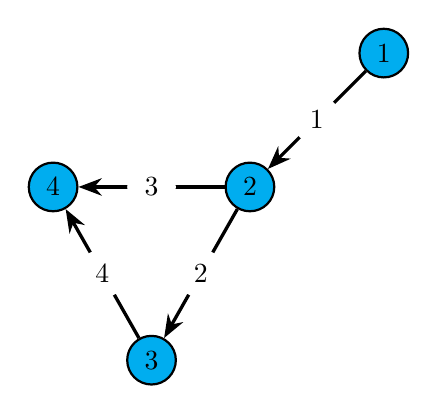
\begin{tikzpicture}
    \begin{scope}[every node/.style={circle,thick,draw,fill=cyan}]%text=white}]
      \node (4) at (0,2.5) {4};
      \node (2) at (2.5,2.5) {2};
      \node (3) at (1.25,.3) {3};
      \node (1) at (4.2,4.2) {1};
    \end{scope}

    \begin{scope}[>={Stealth[black]},
        every node/.style={fill=white,circle},
        every edge/.style={draw=black,very thick}]
      \path [->] (1) edge node {1} (2);
      \path [->] (2) edge node {2} (3);
      \path [->] (3) edge node {4} (4);
      \path [->] (2) edge node {3} (4);
    \end{scope}
  \end{tikzpicture}
\end{columns}


\end{frame}



\begin{frame}
  \frametitle{Framing the load flow problem}

  Suppose we have $N$ nodes labelled by $i$, and $L$ edges labelled by
  $\ell$ forming a directed graph $G$.

  Suppose at each node we have a \alert{power imbalance} $p_i$ ($p_i >
  0$ means its generating more than it consumes and $p_i < 0$ means it
  is consuming more than it).

  Since we cannot create or destroy energy (and we're ignoring losses):
  \begin{equation*}
    \sum_i p_i = 0
  \end{equation*}

  \alert{Question}: How do the flows $f_\ell$ in the network relate to the nodal power
  imbalances?

  \alert{Answer}: According to the reactances (generalisation of
  resistance for oscillating voltage/current) and the corresponding
  voltages.

\end{frame}



\begin{frame}
  \frametitle{Kirchhoff's Current Law (KCL)}

  KCL says (in this linear setting) that the nodal power imbalance at
  node $i$ is equal to the sum of direct flows arriving at the
  node. This can be expressed compactly with the incidence matrix

  \begin{equation*}
    p_i = \sum_\ell K_{i\ell} f_\ell \hspace{2cm} \forall i
  \end{equation*}


  Only $N-1$ of these equations are independent for a connected network, since $\sum_i K_{i\ell} = 0$.
\end{frame}


\begin{frame}
  \frametitle{Kirchhoff's Voltage Law (KVL)}

  KVL says that the sum of voltage differences across edges for any
  closed cycle must add up to zero.

  If the voltage angle at any node is given by $\theta_i$ then the voltage difference across edge $\ell$ is
  \begin{equation*}
    \sum_i K_{i\ell} \theta_i
  \end{equation*}

  And Kirchhoff's law can be expressed using the cycle matrix encoding of independent cycles
  \begin{equation*}
    \sum_\ell C_{\ell c} \sum_i K_{i\ell} \theta_i = 0 \hspace{2cm} \forall c
  \end{equation*}

  [Automatic, since we already said KC = 0.]


\end{frame}



\begin{frame}
  \frametitle{Kirchhoff's Voltage Law (KVL)}

  Physics gives us the expression of the flow $f_\ell$ on each line $\ell$ with reactance $x_\ell$ in terms of the voltage angles at the nodes $\theta_i$  (a
  relative of $V = IR$)
  \begin{equation}
    f_\ell = \frac{\theta_i - \theta_j}{x_\ell} = \frac{1}{x_\ell}\sum_{i} K_{i\ell} \theta_i \label{eq:1}
  \end{equation}
      [NB: This restricts the $L$ variables $f_\ell$ to depend only on the $N$ voltage angles $\theta_i$. Since the flow doesn't change under a constant shift $\theta_i \to \theta_i + c$, we can choose   a \alert{slack} or \alert{reference node} such that  $\theta_1 = 0$, so there are only $N-1$ independent variables.]

      \vspace{.5cm}


  KVL now becomes $L-N+1$ binding constraints on the line flows $f_\ell$
  \begin{equation}
    \sum_\ell C_{\ell c} x_\ell f_\ell = 0 \hspace{2cm} \forall c  \label{eq:2}
  \end{equation}
  [NB: Equations \eqref{eq:1} and  \eqref{eq:2} are equivalent and both restrict our $L$ variables $f_\ell$ to an $N-1$ dimensional subspace.]

\end{frame}

\begin{frame}
  \frametitle{Solving the equations via the line flows}

  Now we have $N-1$ equations for the flows $f_\ell$ from KCL:
  \begin{equation*}
    p_i = \sum_\ell K_{i\ell} f_\ell \hspace{2cm}\forall i \in \{ 1, \dots N-1 \}
  \end{equation*}
  and $L-N+1$ equations from KVL:
  \begin{equation*}
    \sum_\ell C_{\ell c} x_\ell f_\ell = 0 \hspace{2cm}\forall c \in \{ 1, \dots L-N+1 \}
  \end{equation*}

  So $L$ independent linear equations for $L$ variables $f_\ell$.

  Can solve with e.g. LU decomposition using specialised sparse solvers, with polynomial complexity in $L$. (For dense matrices complexity $O(L^a)$ where $2 < a < 3$.)

  This formulation is useful for the optimisation later, but we can solve a smaller dimensional linear system with $N-1$ variables using the voltage angles.
\end{frame}

\begin{frame}
  \frametitle{Solving the equations via the voltage angles}

  If we combine
    \begin{equation}
    f_\ell  = \frac{1}{x_\ell}\sum_{i} K_{i\ell} \theta_i \label{eq:3}
  \end{equation}
    with Kirchhoff's Current Law we get
    \begin{equation*}
    p_i = \sum_{\ell} K_{i\ell}f_\ell =   \sum_{\ell} K_{i\ell} \frac{1}{x_\ell}\sum_{j} K_{j\ell} \theta_j
    \end{equation*}
    This is a \alert{weighted Laplacian}. If we write $B_{k\ell}$ for the diagonal matrix with $B_{\ell\ell} = \frac{1}{x_\ell}$ then
    \begin{equation*}
      L = KBK^t
    \end{equation*}
    and we get a \alert{discrete Poisson equation} for the $\theta_i$ sourced by the $p_i$
    \begin{equation*}
      p_i = \sum_{j} L_{ij} \theta_j
    \end{equation*}
    This is a set of $N-1$ sparse linear equations for the $\theta_j$ ($N-1$ since $\sum_i L_{ij} = 0$).
    We can solve this for the $\theta_i$ and then find the flows using equation \eqref{eq:3}. Polynomial complexity in $N$.

\end{frame}


\begin{frame}
  \frametitle{Solving the equations via the PTDF}

  If we are repeating the calculation for a fixed network multiple times with different power injections, it can make sense to do the full matrix inversion.

  Given $p_i$ at every node, we want to find the flows $f_\ell$. We
  have the equations
    \begin{align*}
      p_i & = \sum_{j} L_{ij} \theta_j \\
     f_\ell  & = \frac{1}{x_\ell}\sum_{i} K_{i\ell} \theta_i
    \end{align*}

    Basic idea: invert $L$ to get $\theta_i$ in terms of $p_i$
    \begin{equation*}
      \theta_i  = \sum_{k} (L^{-1})_{ik} p_k
    \end{equation*}
    then insert to get the flows as a linear function of the power injections $p_i$
    \begin{equation*}
    f_\ell   = \frac{1}{x_\ell}\sum_{i,k} K_{i\ell}  (L^{-1})_{ik} p_k = \sum_k \textrm{PTDF}_{\ell k} p_k
    \end{equation*}
    called the \alert{Power Transfer Distribution Factors} (PTDF).

\end{frame}


\begin{frame}
  \frametitle{Inverting Laplacian $L$}

  There is one small catch: $L$ is \alert{not invertible} since we saw last
  time it has (for a connected network) one zero eigenvalue, with
  eigenvector $(1,1, \dots 1)$, since by construction $\sum_j L_{ij} =
  0$.

  This is related to a gauge freedom to add a constant to all voltage angles
  \begin{equation*}
    \theta_i \to \theta_i + c
  \end{equation*}
  which does not affect physical quantities:
    \begin{align*}
      p_i & = \sum_{j} L_{ij} (\theta_j+ c) = \sum_{j} L_{ij} (\theta_j)  \\
     f_\ell  & = \frac{1}{x_\ell}\sum_{i} K_{i\ell}( \theta_i  + c) = \frac{1}{x_\ell}\sum_{i} K_{i\ell}( \theta_i )
    \end{align*}

    Typically choose a \alert{slack} or \alert{reference node} such that  $\theta_1 = 0$.


\end{frame}

\begin{frame}
  \frametitle{Inverting Laplacian $L$}

  Two solutions:

  1. Since $\theta_1 = 0$ and $p_1$ is not independent of the other
  power injections ($\sum_{i=1}^N p_i = 0$ implies $p_1 = -
  \sum_{i=2}^N p_i$), we can ignore these elements and invert
  the lower-right $(N-1) \times (N-1)$ part of $L$ (which doesn't have zero eigenvalues) to find the
  remaining $\{\theta_i\}_{i=2,\dots N}$ in terms of the
  $\{p_i\}_{i=2,\dots N}$.

  2. Use the Moore-Penrose pseudo-inverse.

  Write $L$ in terms of its basis of orthonormal eigenvectors $e^n_i$ ($\sum_j L_{ij} e^n_j = \l_n e^n_i$, $\sum_i e^n_i e^n_i = 1$ and  $\sum_i e^n_i e^m_i = 0$ if $n \neq m$):
  \begin{equation*}
    L_{ij} = \sum_n \l_n e^n_i e^n_j
  \end{equation*}
  then the Moore-Penrose pseudo-inverse is:
  \begin{equation*}
    L^\dagger_{ij} = \sum_{n | \l_n \neq 0} \frac{1}{\l_n} e^n_i e^n_j
  \end{equation*}



\end{frame}



\begin{frame}
  \frametitle{Check the Moore-Penrose pseudo-inverse}

  Let's check the Moore-Penrose pseudo-inverse really gives us an inverse:
  \begin{align*}
    \sum_{j} L_{ij}L^\dagger_{jk} &= \sum_j \sum_n \l_n e^n_i e^n_j  \sum_{m | \l_m \neq 0} \frac{1}{\l_m} e^m_j e^m_k \\
&= \sum_n \l_n e^n_i  \sum_{m | \l_m \neq 0} \frac{1}{\l_m} e^m_k \sum_j   e^n_j e^m_j \\
    & =   \sum_{m | \l_m \neq 0} \frac{\l_m}{\l_m} e^m_i e^m_k\\
    & =   \sum_{m | \l_m \neq 0}  e^m_i e^m_k
  \end{align*}
  From line 2 to 3 we use the orthogonality of the eigenvectors.

  This is almost the identity. It has eigenvalues 1 for each eigenvector $e^n_k$ except for zero eigenvectors of $L$ with $\l_n = 0$, which it annihilates.

\end{frame}



\begin{frame}
  \frametitle{4-node example}

  \begin{columns}
\column[c]{.5\textwidth}
\begin{equation*}
\mathbf{K}_{i \ell}=\left(\begin{matrix}
1 & 0 & 0 & 0\\
-1 & 1 & 1 & 0\\
0 & -1 & 0 & 1\\
0 & 0 & -1 & -1
\end{matrix}\right)
\end{equation*}
\begin{equation*}
\mathbf{L}_{ij}=\left(\begin{matrix}
1 & -1 & 0 & 0\\
-1 & 3 & -1 & -1\\
0 & -1 & 2 & -1\\
0 & -1 & -1 & 2
\end{matrix}\right)
\end{equation*}
\begin{equation*}
\mathbf{PTDF}_{\ell i}=\left(\begin{matrix}
0 & -1 & -1 & -1\\
0 & 0 & -2/3 & -1/3\\
0 & 0 & -1/3 & -2/3\\
0 & 0 & 1/3 & -1/3
\end{matrix}\right)
\end{equation*}

\column[c]{.5\textwidth}

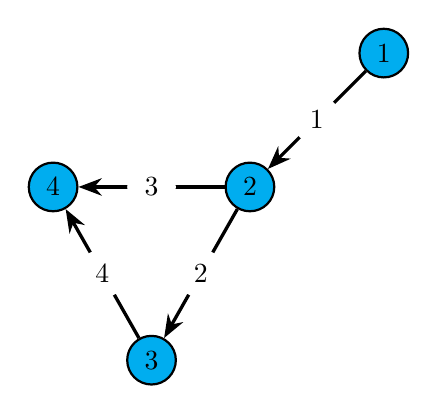
\begin{tikzpicture}
    \begin{scope}[every node/.style={circle,thick,draw,fill=cyan}]%text=white}]
      \node (4) at (0,2.5) {4};
      \node (2) at (2.5,2.5) {2};
      \node (3) at (1.25,.3) {3};
      \node (1) at (4.2,4.2) {1};
    \end{scope}

    \begin{scope}[>={Stealth[black]},
        every node/.style={fill=white,circle},
        every edge/.style={draw=black,very thick}]
      \path [->] (1) edge node {1} (2);
      \path [->] (2) edge node {2} (3);
      \path [->] (3) edge node {4} (4);
      \path [->] (2) edge node {3} (4);
    \end{scope}
  \end{tikzpicture}
\end{columns}


\end{frame}




\begin{frame}
  \frametitle{4-node example}

  \begin{columns}
\column[c]{.65\textwidth}
\begin{align*}
\sum_i \mathbf{PTDF}_{\ell i}p_i & =\left(\begin{matrix}
0 & -1 & -1 & -1\\
0 & 0 & -2/3 & -1/3\\
0 & 0 & -1/3 & -2/3\\
0 & 0 & 1/3 & -1/3
\end{matrix}\right)\left(\begin{matrix}
50\\
50 \\
0\\
-100
\end{matrix}\right) \\
& =\left(\begin{matrix}
50\\
33.3 \\
66.7 \\
33.3
\end{matrix}\right)
\end{align*}

\column[c]{.35\textwidth}

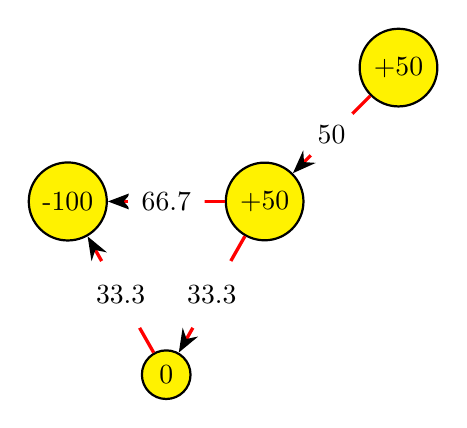
\begin{tikzpicture}
    \begin{scope}[every node/.style={circle,thick,draw,fill=yellow}]
      \node (4) at (0,2.5) {-100};
      \node (2) at (2.5,2.5) {+50};
      \node (3) at (1.25,.3) {0};
      \node (1) at (4.2,4.2) {+50};
    \end{scope}

    \begin{scope}[>={Stealth[black]},
                every node/.style={fill=white,circle},
        every edge/.style={draw=red,very thick}]
      \path [->] (1) edge node {50} (2);
      \path [->] (2) edge node {33.3} (3);
      \path [->] (3) edge node {33.3} (4);
      \path [->] (2) edge node {66.7} (4);
    \end{scope}
  \end{tikzpicture}
\end{columns}


\end{frame}




\begin{frame}
  \frametitle{PTDF as sensitivity}

  Can also `experimentally' determine the Power Transfer Distribution
  Factors (PTDF) by choosing a slack node (in this case node 1).

  Each column (labelled by $i$) is then the resulting line flows if we have
  a simple power transfer from node $i$ to the slack $p_i = 1$ and $p_1
  = -1$.

  \begin{columns}
\column[c]{.5\textwidth}
\begin{equation*}
\mathbf{PTDF}_{\ell i}=\left(\begin{matrix}
0 & -1 & -1 & -1\\
0 & 0 & -2/3 & -1/3\\
0 & 0 & -1/3 & -2/3\\
0 & 0 & 1/3 & -1/3
\end{matrix}\right)
\end{equation*}

\column[c]{.5\textwidth}
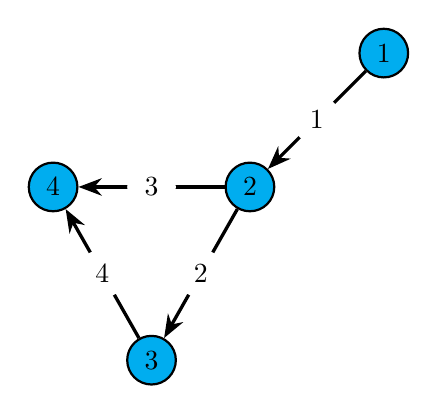
\begin{tikzpicture}
    \begin{scope}[every node/.style={circle,thick,draw,fill=cyan}]%text=white}]
      \node (4) at (0,2.5) {4};
      \node (2) at (2.5,2.5) {2};
      \node (3) at (1.25,.3) {3};
      \node (1) at (4.2,4.2) {1};
    \end{scope}

    \begin{scope}[>={Stealth[black]},
        every node/.style={fill=white,circle},
        every edge/.style={draw=black,very thick}]
      \path [->] (1) edge node {1} (2);
      \path [->] (2) edge node {2} (3);
      \path [->] (3) edge node {4} (4);
      \path [->] (2) edge node {3} (4);
    \end{scope}
  \end{tikzpicture}

\end{columns}


\end{frame}


\begin{frame}
  \frametitle{PTDF as sensitivity: example of 3rd column for node 3}
  \begin{columns}
    \column[c]{.5\textwidth}
    Focus on 3rd column of PTDF and look at power flow with $p_3 = +1$ and slack $p_1 = -1$. Coefficients determined by resulting flow:
\begin{equation*}
\mathbf{PTDF}_{\ell 3}=\left(\begin{matrix}
 &  & -1 &\\
 &  & -2/3 & \\
 &  & -1/3 & \\
 &  & 1/3 &
\end{matrix}\right)
\end{equation*}

\column[c]{.5\textwidth}

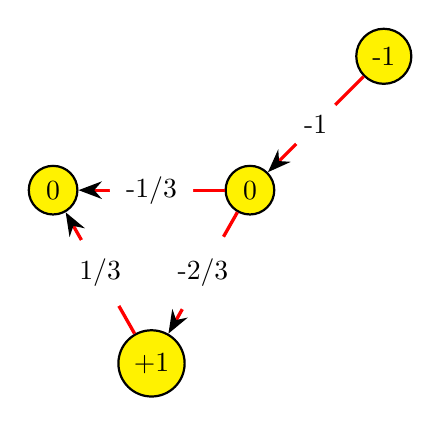
\begin{tikzpicture}
    \begin{scope}[every node/.style={circle,thick,draw,fill=yellow}]
      \node (4) at (0,2.5) {0};
      \node (2) at (2.5,2.5) {0};
      \node (3) at (1.25,.3) {+1};
      \node (1) at (4.2,4.2) {-1};
    \end{scope}

    \begin{scope}[>={Stealth[black]},
                every node/.style={fill=white,circle},
        every edge/.style={draw=red,very thick}]
      \path [->] (1) edge node {-1} (2);
      \path [->] (2) edge node {-2/3} (3);
      \path [->] (3) edge node {1/3} (4);
      \path [->] (2) edge node {-1/3} (4);
    \end{scope}
  \end{tikzpicture}
\end{columns}


\end{frame}


\section{Consequences of limiting power transfers}


\begin{frame}
  \frametitle{Line loading limits}

  You cannot pass infinite current through a transmission line.

  As it warms, it sags, then it will become damaged and/or hit a
  building/tree and cause a short-circuit. For this reasons there are
  always \alert{thermal limits} on current transfer. There may also be
  limits on the amount of power or current based on concerns about
  \alert{voltage stability} or \alert{general stability}.

  Typically each line has a well-defined \alert{line loading limit} on the
  amount of current or power that can flow through it:
  \begin{equation*}
    | f_{\ell } | \leq F_\ell
  \end{equation*}
  where here $F_\ell$ is the maximum power capacity of the transmission line.

  These limits prevent the transfer of renewable energy or other power sources.

\end{frame}




\begin{frame}
  \frametitle{Adjusting generator dispatch to avoid overloading}

  To avoid overloading the power lines, we must adjust our generator
  output (or the demand) so that the power imbalances do not overload
  the network.

  We will now generalise and adjust our notation.

  From lecture 3 we had for a single node:
  \begin{equation*}
    - p_t = m_t -b_t + c_t = d_t - Ww_t - Ss_t -b_t + c_t = 0
  \end{equation*}
  where $p_t$ was the nodal power balance, $m_t$ was the mismatch
  (load $d_t$ minus wind $Ww_t$ and solar $Ss_t$), $b_t$ was the
  backup power and $c_t$ was curtailment.

  We generalised this to multiple nodes labelled by $i$
  \begin{equation*}
    - p_{i,t} = m_{i,t} -b_{i,t} + c_{i,t} = d_{i,t} - W_iw_{i,t} - S_is_{i,t} -b_{i,t} + c_{i,t}
  \end{equation*}
  where now we don't enforce $p_{i,t} = 0$ but $\sum_{i} p_{i,t} = 0$ for
  all $t$.

\end{frame}


\begin{frame}
  \frametitle{Adjusting generator dispatch to avoid overloading} Now
  we write the dispatch of all generators at node $i$ (wind, solar,
  backup) labelled by technology $s$ as $g_{i,s,t}$ ($i$ labels node, $s$ technology and $t$ time) so that we have a relation between load $d_{i,t}$, generation $g_{i,s,t}$ and network flows $f_{\ell,t}$
  \begin{equation*}
    p_{i,t} = \sum_{s} g_{i,s,t} - d_{i,t} = \sum_{\ell} K_{i\ell} f_{\ell,t}
  \end{equation*}
  Where $s$ runs over the wind, solar and backup capacity generators
  (e.g. hydro or natural gas) at the node.

  A dispatchable generator's $g_{i,s,t}$ output can be controlled
  within the limits of its power capacity $G_{i,s}$
  \begin{equation*}
      0 \leq g_{i,s,t} \leq  G_{i,s}
  \end{equation*}
\end{frame}



\begin{frame}
  \frametitle{Variable generation constraints}

  For a renewable generator we have time series of availability $0\leq G_{i,s,t}\leq 1$ (the $s_t$ and $w_t$ before; $W$ and $S$ are the capacity $G_{i,s}$):
    \begin{equation*}
      0 \leq g_{i,s,t} \leq G_{i,s,t} G_{i,s} \leq  G_{i,s}
    \end{equation*}
    Curtailment corresponds to the case where $g_{i,s,t} < G_{i,s,t} G_{i,s}$:

     \centering
  \begin{tikzpicture}
\node[anchor=south west,inner sep=0] (image) at (0,0) {\includegraphics[width=10cm]{scigrid-curtailment}};
\draw (3,2.75) node{$g_{i,s,t}$};
\draw (3,3.4) node{$G_{i,s,t}G_{i,s}$};
\draw (3,4.7) node{$G_{i,s}$};
  \end{tikzpicture}

\end{frame}

\begin{frame}
  \frametitle{Germany curtailment example}

  See \url{https://pypsa.org/examples/scigrid-lopf-then-pf.html}.

\end{frame}


\begin{frame}
  \frametitle{European transmission versus backup energy}

  Consider backup energy in a simplified European grid:

  \centering
  \includegraphics[trim=0 4cm 0 4cm,width=9cm,clip=true]{europe_map}

\end{frame}



\begin{frame}
  \frametitle{DE versus EU backup energy from last time}

  Germany needed backup generation for 31\% of total load:

  \centering
  \includegraphics[width=6.3cm]{mismatch-duration-DE}

  \raggedright
  Europe needed Backup generation for only 24\% of the total load:

  \centering
  \includegraphics[width=6.3cm]{mismatch-duration-EU}

\end{frame}


\begin{frame}
  \frametitle{European transmission versus backup energy}

  \href{http://www.sciencedirect.com/science/article/pii/S0960148113005351}{Transmission needs across a fully renewable European power system} by Rodriguez, Becker, Andresen, Heide, Greiner, Renewable Energy, 2014

  \centering
  \includegraphics[width=6cm]{sarah_balancing.png}


\end{frame}

\end{document}
